%!TEX root = ../thesis.tex

\section{実験の目的}

  本研究では,2DLiDARの反射強度を利用したルールベース制御器を用いた人追従行動を,カメラ画像で模倣学習することを課題としている.ルールベース制御器は,最大反射強度の方向にロボットが追従する手法となっているため,実験で使用する再帰反射テープよりも高い反射強度を検出してしまうと人追従行動を継続できないおそれがある.そのため,実験場所である,千葉工業大学津田沼キャンパス2号館3階(\figref{Fig:RobotGuidance_cit3f})において,再帰反射テープよりも反射強度の高いものが存在しないかを,実験により調査する.

\vspace{2cm}

  \begin{figure}[h]
    \centering
    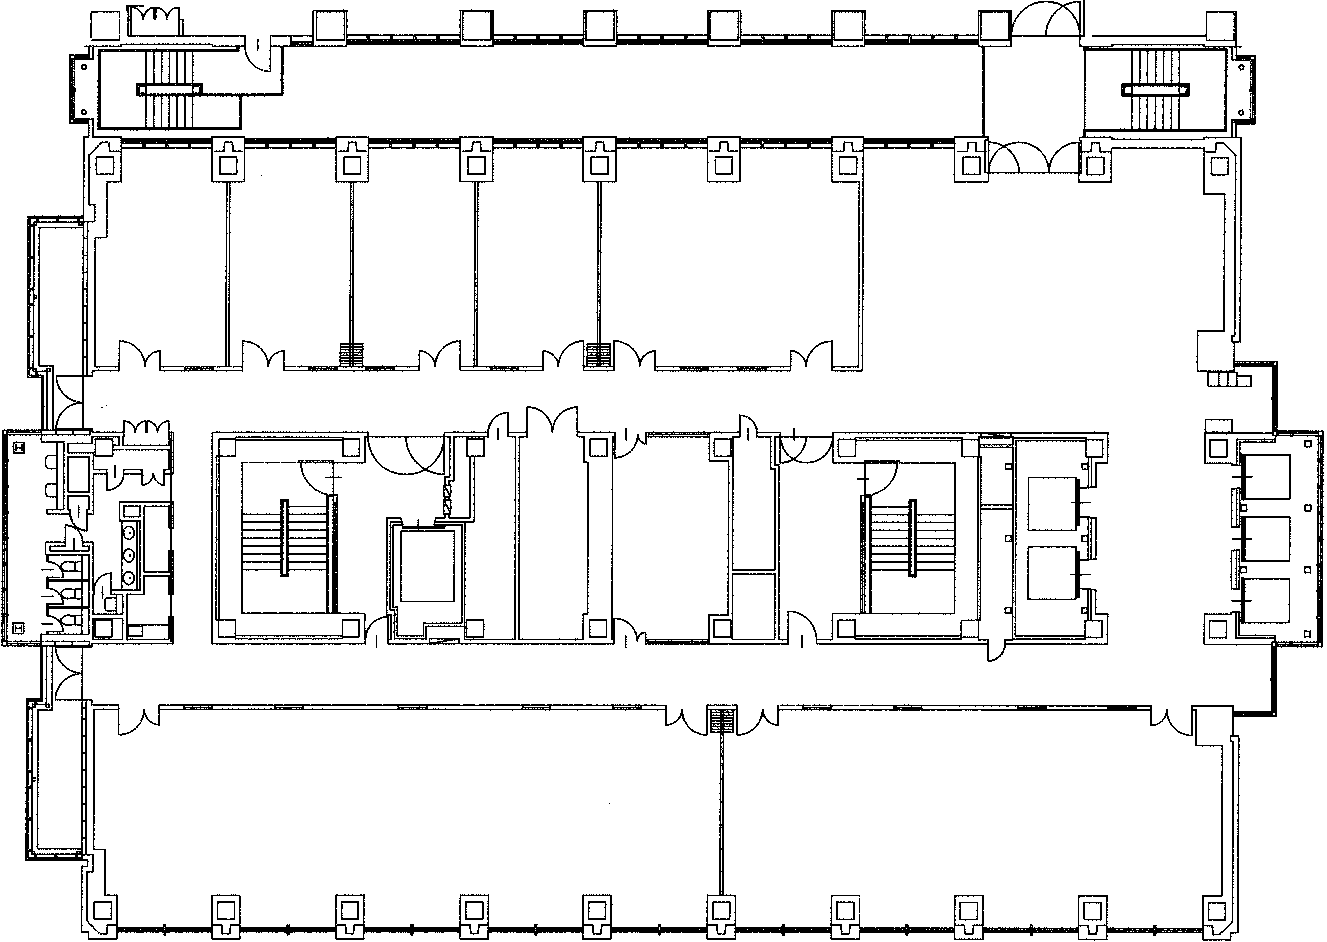
\includegraphics[width=9cm] {images/pdf/RobotGuidance_cit3f}
    \captionsetup{justification=raggedright} % キャプションを左寄せに
    \caption{The environment of the experiment}
    \label{Fig:RobotGuidance_cit3f}
  \end{figure}

\newpage